\chapter{Technical preliminaries}

The chapter has the goal of introducing the math and theory behind
formal languages, parsers, algebra, (zero knowledge) proofs of
knowledge.

\section{Formal Languages \cite{Hopcroft}}

\begin{defn}[Alphabet]
  An alphabet $\Sigma$ is a set of symbols.
\end{defn}

\begin{defn}[String]
  A string over an alphabet $\Sigma$ is a sequence of symbols of $\Sigma$.
\end{defn}

\begin{defn}[Concatenation]
  Let $x = a_0 a_1 \dotsm a_n$ and $y = b_0 b_1 \dotsm b_n$, then the
  string $x y = a_0 a_1 \dotsm a_n b_0 b_1 \dotsm b_n$ is the
  concatenation of the strings $x$ and $y$.
\end{defn}

\begin{defn}[Sets]
  The $\Sigma^*$ denotes the set of all the strings over the alphabet
  $\Sigma$, likewise $\Sigma^+$ denotes the set of all the non-empty
  strings over the alphabet $\Sigma$. $$\Sigma^+ \subseteq \Sigma^*
  \setminus \{ \epsilon \}$$ The empty set of strings is denoted
  $\emptyset$.
\end{defn}

\begin{defn}[Language]
  A language over the alphabet $\Sigma$ is a set of strings over
  $\Sigma$. Members of the language are called words of the language.
\end{defn}

\begin{defn}[Concatenation]
  Let $L_1$ and $L_2$ be two languages over alphabet $\Sigma$, the
  language $L_1 L_2 = \{x y | x \in L_1, y \in L_2 \}$ is the
  concatenation of $L_1$ and $L_2$.
\end{defn}

\begin{defn}[Kleene closure]
  Let $L$ be a language over $\Sigma$. Define 
  $$L^0 = \{ \epsilon \}$$
  $$L^i = L L^{i-1} \textrm{for} i \ge 1$$
  the \emph{Kleene closure} of $L$, denoted by $L^*$ is the language:
  $$ L^* = \bigcup_{i \ge 0} L^i $$
  the \emph{positive closure} is
  $$ L^+ = \bigcup_{i \ge 1} L^i $$
  It can be observed that
  $$ L^* = L^+ \cup \{ \epsilon \} $$
  $$ L^+ = L L^* $$
\end{defn}

\subsection{Regular expression}

\begin{defn}[Regular expression]
  A regular expression over $\Sigma$ is defined inductively as follows:
  \begin{enumerate}
  \item $\emptyset$ is a regular expression and represents the empty language
  \item $\epsilon$ is a regular expression and represents the language
    $L = \{ \epsilon \}$
  \item For each $c \in \Sigma$, $c$ is a regular expression and
    represents the language $L = \{ c \}$
  \item For any regular expressions $r$ of language $R$ and $s$ of language $S$:
    \begin{itemize}
    \item $r+s$ is a regular expression representing language $R \cup S$
    \item $r s$ is a regular expression representing language $R S$
    \item $r^*$ is a regular expression representing language $R^*$
    \item $r^+$ is a regular expression representing language $R^+$
    \end{itemize}
  \end{enumerate}
\end{defn}

\begin{thm}
  $r r^*$ can be represented as $r+$
\end{thm}

\begin{proof}
  $r r^*$ represents the language $R R^*$ which is $R^+$
\end{proof}

\subsection{Grammars}

\begin{defn}[Grammar]
  A grammar is a 4-tuple $G = \left< \Sigma, V, S, P \right>$:
  \begin{enumerate}
  \item $\Sigma$ is a finite non-empty set called the \emph{terminal
    alphabet}. The elements of $\Sigma$ are called \emph{terminals}.
  \item $V$ is a finite non-empty set disjoint from $\Sigma$. The
    elements of $V$ are called \emph{non-terminals} or \emph{variables}.
  \item $S \in V$ is a distinguished symbol called the \emph{start symbol}
  \item $P$ is a finite set of \emph{productions (rules)} of the form
    $$ \alpha \rightarrow \beta $$
    $$ \alpha \in (\Sigma \cup V)^* V (\Sigma \cup V)^* $$
    $$ \beta \in (\Sigma \cup V)^* $$
  \end{enumerate}
\end{defn}

\begin{defn}[Context-free grammar]
  The grammar $G$ is a context free grammar if $|\alpha|$ = 1 ($\alpha = V$).
\end{defn}

\begin{defn}[LL grammar]
  A context free grammar $G$ is an LL grammar if $\beta \in \Sigma
  (\Sigma \cup V)^*$
\end{defn}

\section{Montgomery Product}

Modular multiplications would involve trial division after the
multiplication step were it not for the algorithm know as Montgomery
product invented by Peter L. Montgomery \cite{Montgomery}.

The basic step and the property of the algorithm is computing the
residues modulo $N$.

\begin{defn}
  Define an radix $R$ such that $R R^{-1} - N N' = 1$. The residue
  $\overline{a}$ of $a$ is $\overline{a} = a R$
\end{defn}

\begin{thm}
  The algorithm for Montgomery reduction is
  \begin{algorithm}[hbt!]
    \caption{Montgomery reduction}
    \begin{algorithmic}
      \Function{Reduce}{$T$}
      \State $m \gets (T \bmod{R}) N' \bmod{R}$
      \State $t \gets (T + m N)/R$
      \If{$t \ge N$} \Return $t - N$
      \Else \, \Return $t$
      \EndIf
      \EndFunction
    \end{algorithmic}
  \end{algorithm}
\end{thm}
\begin{proof}
  Assume $T < R$, then
  \begin{align*}
      m & = T N' \\
    m N & = T N' N \\
        & = T R R^{-1} - T \\
        & = - T \bmod{R} \\
    t R & = T + m N \\
        & = T \bmod{N}
  \end{align*}
\end{proof}

To compute the Montgomery product, one can now apply the reduction to
the product of the reduced $\overline{a}$ and $\overline{b}$:
\begin{algorithmic}
  \Function{MontgomeryProduct}{$\overline{a}$, $\overline{b}$}
    \State $t \gets \overline{a} \cdot \overline{b}$
    \State \Return \Call{Reduce}{$t$}
  \EndFunction
\end{algorithmic}

Ko\c{c} goes a step further and inlines the reduction to see possible
optimizations when implementing the algorithm on multiple
architectures \cite{Koc}:

\begin{algorithm}[hbt!]
  \begin{algorithmic}
    \Function{MontgomeryProduct}{$\overline{a}$, $\overline{b}$}
      \State $m \gets (\overline{a} \cdot \overline{b} \bmod{R}) N' \bmod{R}$
      \State $t \gets (\overline{a} \cdot \overline{b} + m N)/R$
      \If{$t \ge N$} \Return $t - N$
      \Else \, \Return $t$
      \EndIf 
   \EndFunction
  \end{algorithmic}
\end{algorithm}

If such a primitive is provided on an architecture, the reduction then
becomes:

\begin{algorithm}
  \begin{algorithmic}
    \Function{MontgomeryReduce}{$T$}
      \State \Return \Call{MontgomeryProduct}{$T$, $R^2$}
    \EndFunction
  \end{algorithmic}
\end{algorithm}

Montgomery product eliminates the trial division. It does so at the
expense of computing the residues. However, these residues can be
precomputed in the beginning. Then, for a sufficient number of
Montgomery multiplications, the amortized cost is negligible. The
problem of computing the modular product is then given by:
\begin{enumerate}
\item Transform into the Montgomery domain
\item Compute the product in the Montgomery domain
\item Transform the result back into the integer domain
\end{enumerate}
This is also depicted in Figure \ref{fig:montpro_flow} where both paths
are shown when starting from the integer domain.

\begin{figure}[hbt!]
  \centering
  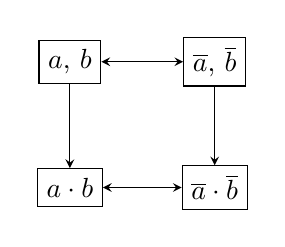
\begin{tikzpicture}[>=stealth]
    \tikzstyle{dom}=[rectangle,draw=black,thin,align=center]

    \node[matrix, column sep=1cm, row sep=1cm](matrix){
      \node[dom](intd){$a$, $b$}; & \node[dom](montd){$\overline{a}$, $\overline{b}$}; \\
      \node[dom](intpro){$a \cdot b$}; &\node[dom](montpro){$\overline{a} \cdot \overline{b}$}; \\
    };

    \draw[<->] (intd) -- (montd);
    \draw[->] (montd) -- (montpro);
    \draw[<->] (montpro) -- (intpro);
    \draw[->] (intd) -- (intpro);
  \end{tikzpicture}
  \caption{Montgomery product flow}
  \label{fig:montpro_flow}
\end{figure}

\filbreak

\section{Turing Machine}

A Turing machine is a mathematical model of computation \cite{Turing}.
Informally, it consists of:
\begin{itemize}
\item A tape divided into cells
\item A head that reads and writes
\item A finite table (action table or transition function)
\item A state
\end{itemize}

\begin{figure}[hbt!]
\centering
\begin{tikzpicture}[
      start chain=1 going right,start chain=2 going below,node distance=-0.15mm
    ]
    \node [on chain=2] {Tape};
    \node [on chain=1] at (-1.5,-.4) {\ldots};  
    \foreach \x in {1,2,...,11} {
        \x, \node [draw,on chain=1] {};
    } 
    \node [name=r,on chain=1] {\ldots}; 
    \node [name=k, arrow box, draw,on chain=2,
        arrow box arrows={east:.25cm, west:0.25cm}] at (-0.335,-.65) {};    
    \node at (1.5,-.85) {Read/write head};
    \node [on chain=2] {};
    \node [draw,on chain=2] {Program};
    \chainin (k) [join];
\end{tikzpicture}
\caption{Turing machine}
\label{fig:turing}
\end{figure}

A more formal definition comes from Hopcroft \cite{Hopcroft}. A Turing machine
is defined as a 7-tuple $M = \left< Q, \Gamma, b, \Sigma, q_0, F, \delta \right>$
\begin{itemize}
\item $Q$ is a finite, non-empty set of states
\item $\Gamma$ is a finite, non-empty set of the tape alphabet/symbols
\item $b \in \Gamma$ is the blank smybol
\item $\Sigma \subseteq \Gamma \setminus \{ b \}$ the set of input symbols
\item $q_0 \in Q$ is the initial state
\item $F \subseteq Q$ is the set of final or accepting states
\item $\delta : Q \setminus F \times \Gamma \rightarrow Q \times \Gamma \times \{ L,R \}$ is the transition relation
\end{itemize}

\section{Zero Knowledge Proofs of Knowledge}

Sometimes one party wants to prove knowing a secret to the other party
but without actually revealing that secret. Let's take a corporate
espionage example. Suppose that we wish to buy a secret but are not
convinced of the seller's honesty (he may leave us without money and
run away with our secret). We then devise a protocol by which we can
be convinced that the seller knows the secret.

\filbreak

To define a proof a knowledge it is convenient to use a Turing
machine. In this case let's define an interactive Turing machine (ITM)
with 5 tapes:
\begin{itemize}
\item Input tape (read-only)
\item Receiving tape (read-only)
\item Sending tape (write-only)
\item Output tape (write-only)
\item Working tape (read-write)
\end{itemize}

An interactive protocol is an ordered pair of ITMs that share the same
input tape, and have receiving and sending tapes cross-connected
(sending to receiving, receiving to sending).

An interactive proof system can be represented by the following two
properties:
\begin{itemize}
\item Completeness $(x,w) \in \mathcal{R} \Rightarrow P(accept) > \frac{2}{3}$
\item Soundness $(x,w) \notin \mathcal{R} \Rightarrow P(accept) < \frac{1}{3}$
\end{itemize}

Informally, the previous two properties state that
\begin{itemize}
\item if a statement is true, a honest prover will be able to convince the verifier of the validity with a large probability
\item if a statement is false, no dishonest prover will be able to convince the verifier of the validity with a probability larger than the threshold
\end{itemize}

To make it a zero-knowledge an additional property is needed. We can
state that the prover should not release any knowledge on the secret
it possesses. To make it more formal, we state that a third party
should not be able to distinguish between a successful communication
and an unsuccessful one. Depending on how indistinguishable it is, we
can differentiate three cases:
\begin{itemize}
\item perfectly indistinguishable
\item statistically indistinguishable
\item computationally indistinguishable
\end{itemize}

\section{Data Flow Graph and Control Flow Graph}

An algorithm is completely and uniquely defined by its Data Flow Graph (DFG),
whereas the implementation of an algorithm is what gives it its Control Flow
Graph (CFG).

The usual step in converting an algorithm in software to an algorithm
in hardware is to extract the DFG \cite{Schaumont}.

%%% Local Variables: 
%%% TeX-PDF-mode: t
%%% TeX-master: "thesis"
%%% End: 
